%%%%%%
%
% $Autor: Sudeshna Nanda $
% $Datum: 2024-10-20 $
% $Pfad: ML23-06-Magic-Wand-with-an-Arduino-Nano-33-BLE-sense/manual/Contents/en/SystemRequirements.tex $
% $Version: 1 $
%
%%%%%%



\chapter{Setup Menu}\label{Setup}

\section{Performing the initial setup}

The initial setup differs from model to model.

\subsection{Initial Setup}
The setup menu allows you to access and perform the magic wand.

\subsection{Installation}
Arduino Nano 33 BLE Sense uses the Arduino software integrated development environment (IDE) for programming, which is the most widely used and common (IDE) for all arduino boards that can be run online and offline. This is a open-source Arduino Software (IDE) makes it easy to write code and upload it to the board. There are various version of software which is supported for each operating system (OS) e.g: mac, linux, and windows. Arduino community also provide us to start coding online and save our sketches in the cloud, this online arduino editor is most up-to-date version of the IDE includes all libraries and also supports new Arduino boards. For getting access to these software packages go to the following link \url{https://www.arduino.cc/en/software}  and get more up to date inforamtion, because every single day there are some updates occurs which is available on the link mention above. These software can be used with any Arduino board, the most recent offline arduino IDE 1.8.15 can be seen in Figure,\ref{fig:Arduino Creat Agent Installation}. it is also supportive for all operating systems.


\begin{figure}[h]\centering
	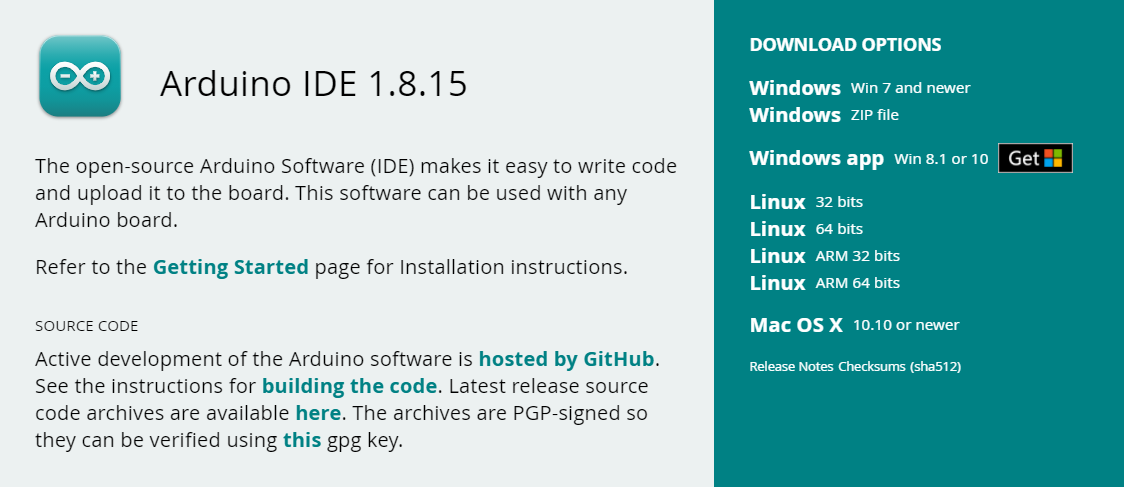
\includegraphics[width=8cm]{Images/SoftwareDescription/Arduino Creat Agent Installation}
	\caption{\textbf{Arduino Creat Agent Installation.}}
	\label{fig:Arduino Creat Agent Installation}		
\end{figure}

\subsection{System Requirement}
\fcolorbox{blue}{blue!10}{\begin{minipage}{\textwidth}
		\begin{center}
			\begin{tabular}{llm{90mm}} 
				%\multicolumn{3}{l}{\large \textcolor{blue}{ Tech Specs of Arduino Nano 33 BLE Sense}} \\ \hline
				\\ \textbf{\MapleCommand{\textcolor{blue}{Operating System}}}  & Windows 7 or above, MacOS X or higher \\
				\textbf{\MapleCommand{\textcolor{blue}{CPU}}}  & Intel i3 or above\\
				\textbf{\MapleCommand{\textcolor{blue}{RAM}}}  & Min 2GB\\
				\textbf{\MapleCommand{\textcolor{blue}{Arduino IDE}}}  & V. 1.1819 \\
				\textbf{\MapleCommand{\textcolor{blue}{Boards}}}  & Arduino mBED OS Nano \\
				\textbf{\MapleCommand{\textcolor{blue}{Libraries}}}  & LSM9DS1 \\
				\textbf{\MapleCommand{\textcolor{blue}{Interface}}}  & USB port \\			
			\end{tabular}
		\end{center}
\end{minipage}}

\subsection{Configuration}
\subsubsection{Configuration for the Arduino Nano 33 BLE Sense}
To program the Arduino Nano 33 BLE Sense in offline state, we need to install one
of the latest arduino IDE on our desktop. After installation, for getting access to
the Arduino nano 33 ble sense board, we need to make configuration in our IDE. By
opening the IDE, go to tool which can be seen on the uper left corner in IDE, in the
tool there is an option for managed board. At this point we need to write our board
name in the search which is Arduino Nano 33 BLE Sense as shown in figure,\ref{fig:Arduino Mbed OS Nano Boards Installation}.Select
the Arduino Mbed OS Boards and install it. The Mbed OS nano board supports also
other nano family boards including Arduino nano 33 ble sense, after installing simply
connect the Arduino Nano 33 BLE Sense to the computer via USB cable.


\begin{figure}[h]\centering
	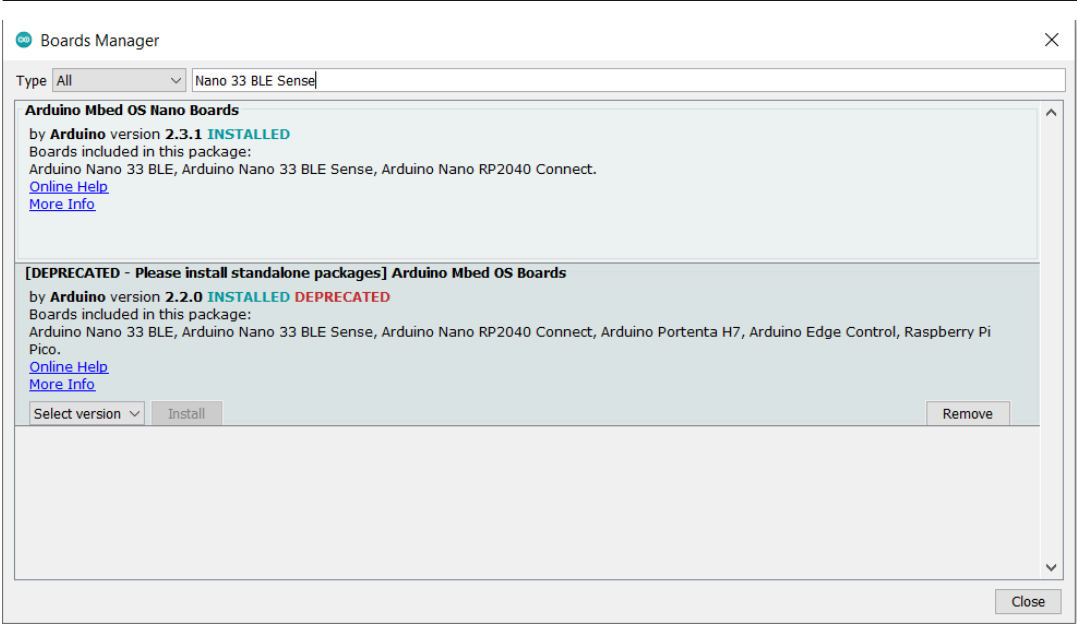
\includegraphics[width=8cm]{Images/SoftwareDescription/Arduino Mbed OS Nano Boards Installation}
	\caption{\textbf{Arduino Mbed OS Nano Boards Installation.}}
	\label{fig:Arduino Mbed OS Nano Boards Installation}		
\end{figure}



\subsection{Setup}
There are set of examples which are build in Arduino (IDE) for the testing purpose, for checking all the configuration and setting up the board we can open one of the basic LED blink example first as shown in the figure.  \ref{fig:LED-Example Test}.



\begin{figure}[h]\centering
	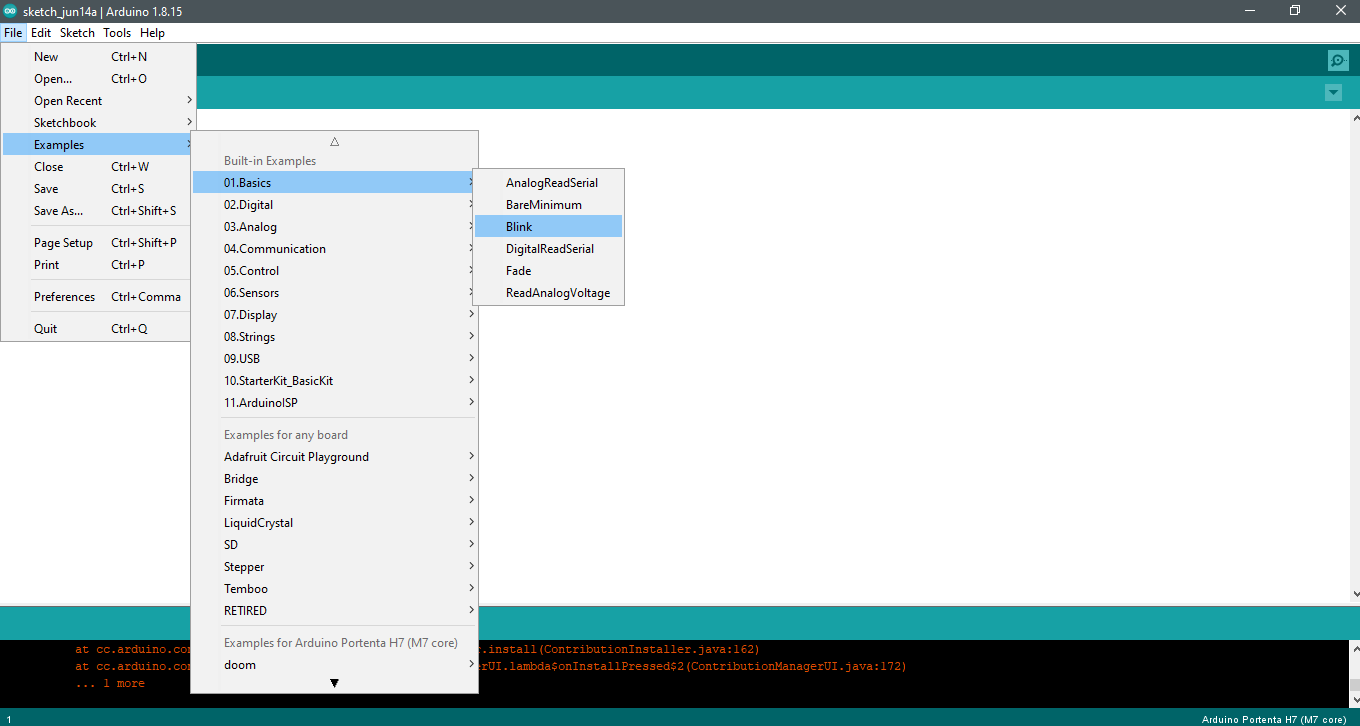
\includegraphics[width=8cm]{Images/SoftwareDescription/Menu bar options}
	\caption{\textbf{LED-Example Test.}}
	\label{fig:LED-Example Test}		
\end{figure}
This LED-blink example support all the arduino boards, for the checking purposes just need to run this basic example on any arduino embed board and it will blink the LED on our Arduino board after pre-set miliseconds. In the same example folder, there are also number of build in usefull example written in Arduino IDE for embedded boards. These examples are very usefull for getting the basic knowledge about the board and programming.

\subsection{Output Window (Serial Monitor)}
Serial Monitor is the another window on the Arduino IDE, which shows the Input/Output of our program and results appear on it as per the required output. For getting
access to Serial monitor, we need to go extreme right in the Arduino IDE, the small
circle pop up when we reach it is the serial monitor as show in the figure.\ref{fig:Serial Monitor Icon}
\begin{figure}[h]\centering
	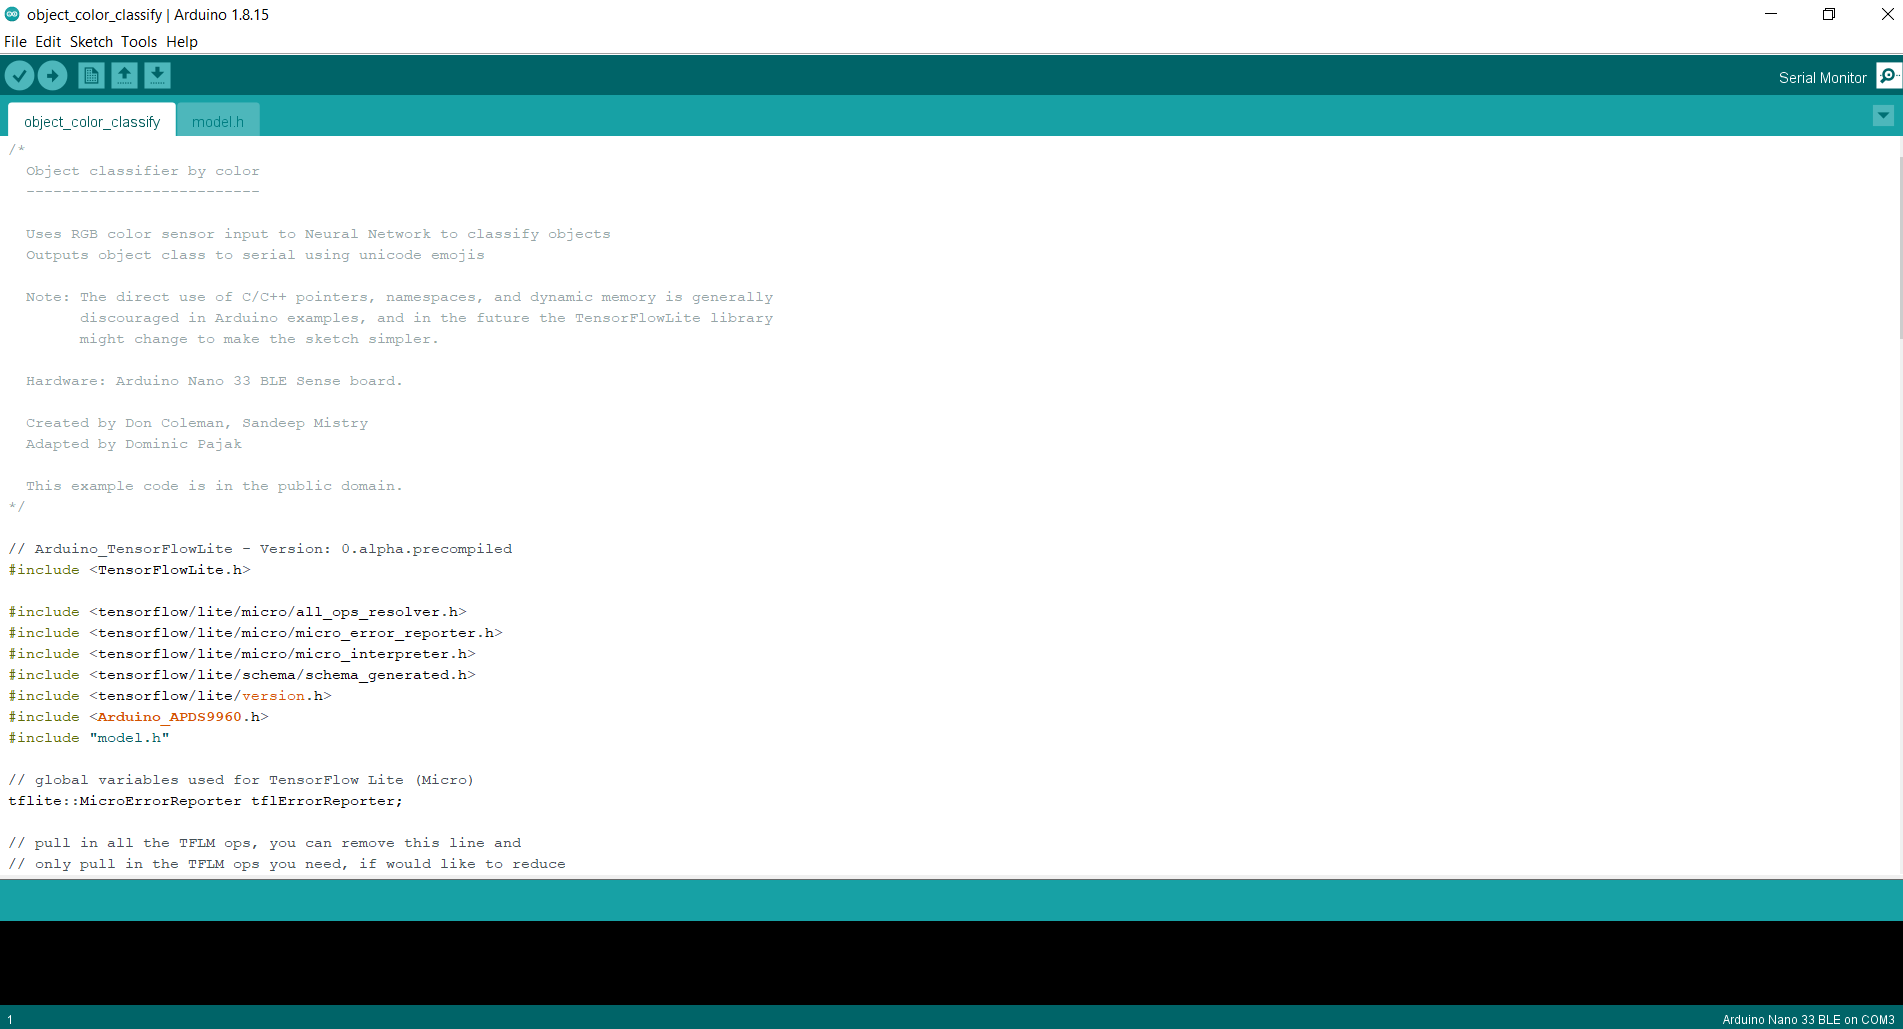
\includegraphics[width=8cm]{Images/SoftwareDescription/Serial Monitor Icon}
	\caption{\textbf{Serial Monitor Icon.}}
	\label{fig:Serial Monitor Icon}		
\end{figure} 
The Final results, all the variables, input, sensor values are shown in the serial monitor
the (Output Window) as shown in the figure\ref{fig:Output Window} by clicking the serial monitor button.
\begin{figure}[h]\centering
	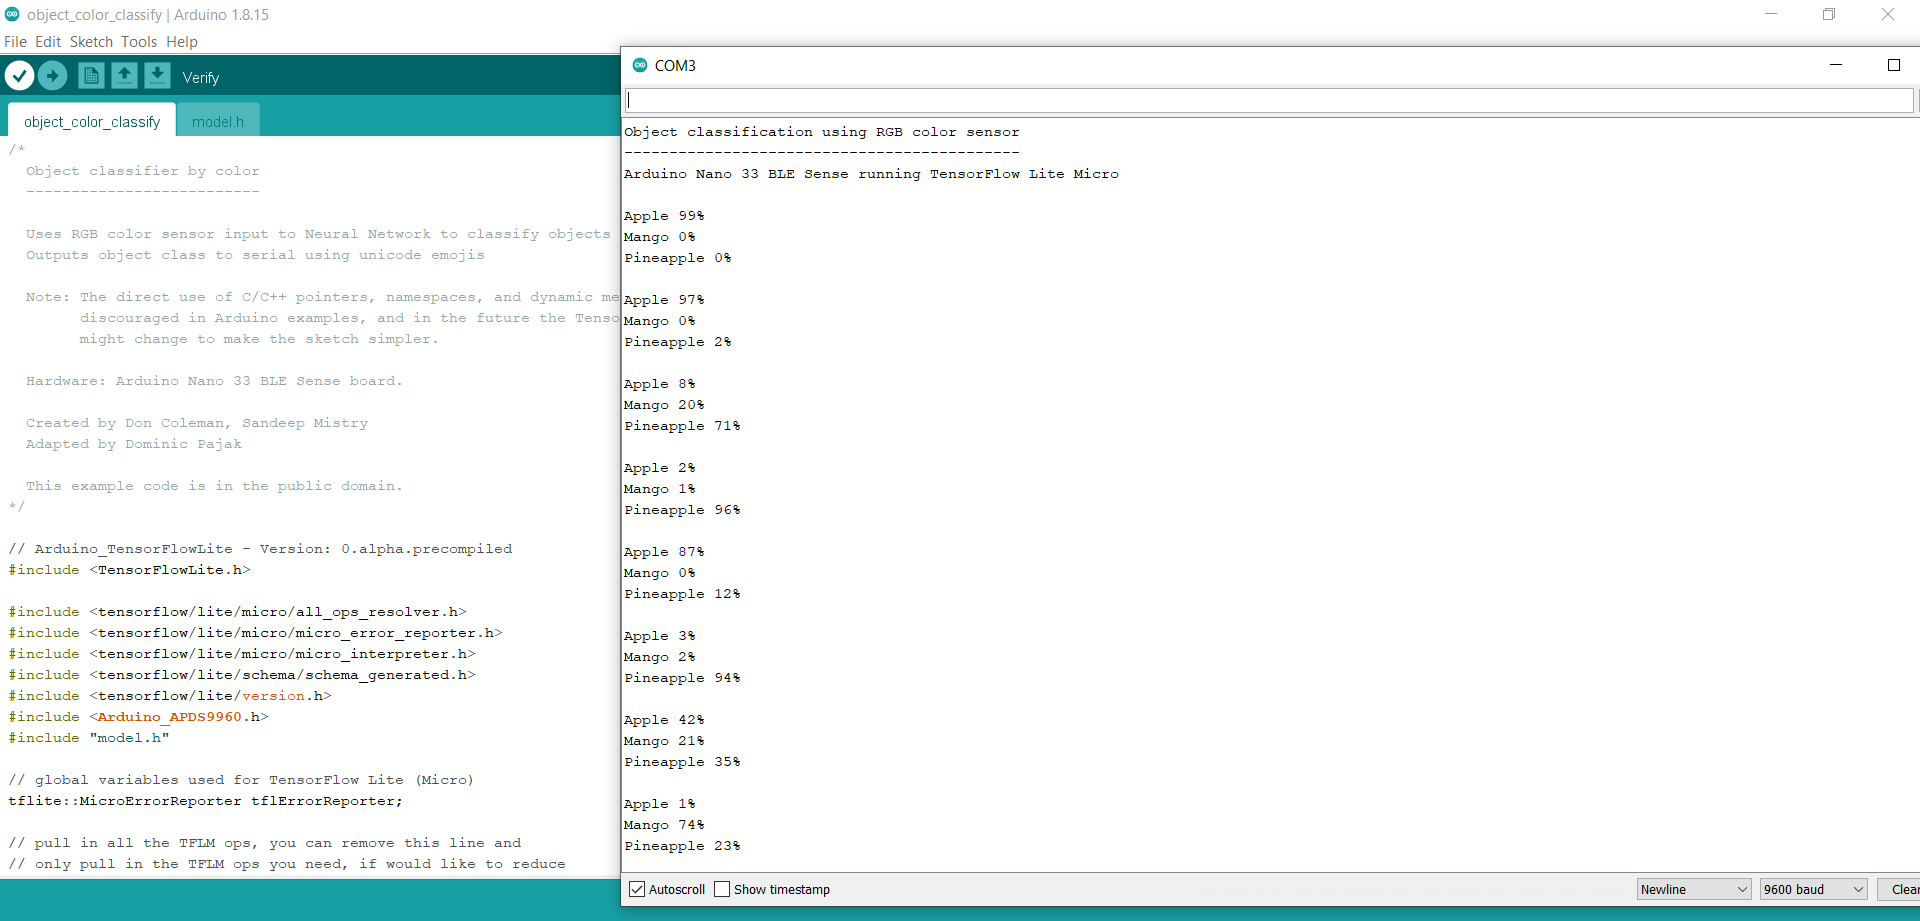
\includegraphics[width=8cm]{Images/SoftwareDescription/Output Window}
	\caption{\textbf{Output Window.}}
	\label{fig:Output Window}		
\end{figure} 
